% paper/main.tex
% Every number below is copied from a file in results/ or notes/; the source is in a comment next to it.
% Red [bracketed] text marks what the author must still write or approve.
\documentclass[12pt]{article}
\usepackage[margin=1in]{geometry}
\usepackage{setspace}\doublespacing
\usepackage{lineno}\linenumbers
\usepackage{graphicx,booktabs,amsmath}
\usepackage{xurl}\usepackage[hidelinks]{hyperref}\sloppy
\usepackage{natbib}\bibliographystyle{apalike}
\usepackage{xcolor}
\newcommand{\todo}[1]{\textcolor{red}{\textbf{[#1]}}}
\graphicspath{{../figures/}}
\pagestyle{plain}

\title{When Does the Undercut Work?\\Pit-Stop Battles in Formula 1, 2023--2026}
\author{Jason Kim}
\date{}

\begin{document}
\maketitle

\begin{abstract}
% sources: results/attempt_counts.csv, rq1_rates.csv, rq1_odds.csv, rq2_loso.csv, rq2_diffs.csv, rq2_rule.csv, rq3_rate.csv, mechanism.csv, rq4_odds.csv, rq4_prepace.csv, rq4_checks.csv
The undercut, where a car stuck behind a rival pits first and uses fresh tyres to jump ahead, is Formula 1's best-known strategy move, yet how often it works has not been measured publicly. Using lap-end timing from every dry Grand Prix from 2023 to round 17 of 2026, we find 177 green-flag undercut attempts: the chasing car was within 3 seconds of the car ahead, pitted first, and the car ahead pitted within five laps. In 2023--25 half of the attempts worked (95\% race-bootstrap CI 41--59\%). Two factors stood out. Each extra second of gap cut the odds of success by 72\%, and the undercut worked 36\% of the time when the car ahead responded on the next lap but 72--75\% when it waited three laps or more. The commentators' rule of thumb (fresh-tyre gain per lap times laps before the response must exceed the gap) points the right way, but as a yes/no call it is overconfident: on held-out seasons its Brier score (0.331) is worse than always predicting the average (0.252). Turned into a probability, the same rule predicts as well as a full logistic model (0.211 vs 0.218). In a typical successful undercut the chaser gained 4.0~s while on fresher tyres and 1.1~s from a slower stop by the rival. In exploratory analyses, neither the chaser's car pace nor its pit-crew record predicted success once the gap was known. In 2026, 36\% of 22 attempts worked; this drop is suggestive but not conclusive.
\end{abstract}

\section{Introduction}

A Formula 1 car that is stuck behind a slightly slower rival has a problem: overtaking on track is hard, and every lap spent in the rival's turbulent air costs time and tyre life. The \emph{undercut} is the standard way out. The chasing car pits first and, on fresh tyres, laps faster than the rival can on worn ones. When the rival pits a lap or two later, the chaser has made up the gap and comes out ahead. ``The undercut is where you pass your rival by pitting before him and being faster on your new tyre out-lap'' \citep{hughes2021undercut}; the chasing driver ``must be within striking range,'' which is ``typically within two seconds'' \citep{palmer2019singapore}.

Television commentary treats the undercut as a known quantity (``the undercut is worth about two seconds here''), but we found no public estimate of how often it actually works, or of what decides it. Strategy research in motorsport has built full race simulations \citep{bekker2009planning,heilmeier2020monte}, neural networks that make pit-stop decisions \citep{heilmeier2020virtual} and game-theoretic models of when to stop \citep{aguad2024pit}. These models need lap-time and tyre models that only teams can calibrate well, and they answer ``what should a team do?'' rather than ``what happens when teams try it?'' In this journal, \citet{weissbock2025qualifying} showed how strongly qualifying position predicts the finish, and listed pit and tyre strategy among the open questions for Formula 1. No paper here has studied pit strategy.

This paper measures the undercut directly. Using free lap-by-lap timing data, we find every attempt in the dry Grands Prix from 2023 to round 17 of 2026 and record whether it worked. We ask four questions:

\begin{itemize}
\item \textbf{RQ1.} How often does the undercut work, and what decides it: the gap before the stop, how quickly the car ahead responds, tyre age, the tyre compound, the time lost in the pit lane, or how fast tyres wear at that circuit?
\item \textbf{RQ2.} Does a statistical model predict whether an undercut will work better than the rule of thumb that commentators use (fresh-tyre gain per lap, times the number of laps before the car ahead responds, must exceed the gap)?
\item \textbf{RQ3 (exploratory).} Did the 2026 rules, which brought new cars and new tyres, change the undercut?
\item \textbf{RQ4 (exploratory).} What kind of team or car closes the gap: a faster car, one that is easier on its tyres, or a quicker pit crew?
\end{itemize}

The paper makes three contributions. It gives the first public, race-by-race estimate of how often the undercut works. It turns the rule of thumb into a testable prediction and shows that, as a yes/no call, the rule is overconfident, while a calibrated version of it predicts as well as a full statistical model. And it splits the time an undercut gains into the part won in the pit lane and the part won on track. All definitions, models and metrics were fixed and tagged in the project's git history before any model was fitted to real data.

\section{Materials and Methods}

\subsection{Data}
% source: data/laps/*_info.json (87 races; wet 4/4/4/3), results/attempt_counts.csv
We use every Grand Prix from 2023 to the 2026 Singapore Grand Prix (round 17): 22 races in 2023, 24 in each of 2024 and 2025, and 17 in 2026, for 87 in total. Sprint races are excluded because they have no compulsory pit stop. Timing data come from the FastF1 Python package \citep{fastf1}, which provides each car's lap times, the time it crossed the timing line at the end of each lap, pit-in and pit-out flags, tyre compound and tyre age, and the track status (green, yellow, safety car, virtual safety car or red flag) on every lap. All data were read from a local cache, so the analysis can be rerun without network access. A race is \emph{wet}, and excluded, if any driver used intermediate or wet tyres or the weather feed recorded rain during the race. This removes 15 races (four in each of 2023--25 and three in 2026), leaving 72 dry races.

\subsection{Undercut attempts}
We measure the gap between two cars with the times at which they cross the timing line at the end of the same lap. Comparing cars on the same lap number means a car that has been lapped is never treated as the car ahead. A pit stop counts only if the car changes tyres: the lap after its pit-in lap must show a different compound or a lower tyre age. Drive-through and stop-go penalties, which keep the same tyres, are therefore not stops.

Car B (the \emph{chaser}) and car A (the \emph{leader}) form an \emph{undercut attempt} when:
\begin{enumerate}
\item on the lap before B's stop (lap $n-1$), A is the car directly ahead of B, and B crosses the line within 3.0~s of A;
\item B makes a real stop on lap $n$, and neither car was in or out of the pits on lap $n-1$, nor was A on lap $n$;
\item A makes a real stop on lap $m$ within the next five laps ($n+1 \le m \le n+5$). The \emph{response delay} is $m-n$ laps;
\item every lap from $n-1$ to the check lap (below) is fully green for both cars, with no yellow flag, safety car, virtual safety car or red flag, and neither car uses intermediate or wet tyres or retires before the check lap.
\end{enumerate}
The attempt \emph{works} if B crosses the line ahead of A at the end of lap $m+2$, the lap after A's out-lap, when both stops are complete. If A does not stop within five laps, the case is a \emph{no response} and is counted but not modelled, because A is then on a different strategy rather than responding.

As robustness checks we repeat the analysis with gap windows of 2~s and 5~s, with the outcome checked one lap later (lap $m+3$), and with the green-flag rule applied only to laps $n-1$ to $m+1$.

To check the detection, ten attempts were drawn at random and each one was checked against the two cars' lap times, pit flags, tyre data and line-crossing times (\texttt{notes/spotcheck.md} in the repository). All ten were correctly identified and correctly labelled.

\subsection{Features}
Each attempt is described by the gap on lap $n-1$; the response delay, grouped as 1, 2, 3 or 4--5 laps; the difference in tyre age between the leader and the chaser on lap $n-1$ (positive when the leader's tyres are older); and the chaser's compound change (to a harder, the same, or a softer compound). The response delay is the leader's choice, made after it has seen the chaser stop, and it is known only once the leader pits. The models in this paper therefore describe and predict the outcome \emph{given} the leader's response; they do not forecast an attempt before the chaser stops. Three more features describe the race, and are measured only on the \emph{other} cars in that race, so that no feature uses the attempt's own outcome:
\begin{itemize}
\item \textbf{Fresh-tyre gain} (s per lap): for each other car's stop within ten laps of lap $n$, the mean of its two laps before the in-lap minus the mean of its two laps after the out-lap, all green. The race value is the median over those stops.
\item \textbf{Pit loss} (s): for each other car's green stop, its in-lap plus out-lap time minus twice its median normal lap time nearby. The race value is the median.
\item \textbf{Tyre wear} (s per lap of tyre age): for each other car's stint of at least six green laps, excluding lap 1 and in- and out-laps, the slope of lap time against tyre age from a straight-line fit. The race value is the median. Because fuel burns off during a stint, this slope is wear net of the fuel effect.
\end{itemize}
One 2026 attempt had no other-car stop within ten laps and therefore no fresh-tyre gain; it is dropped from all models, leaving 176 attempts. % source: analysis/rq1.py output (1 dropped, 2026_10)

\subsection{The rule of thumb}
Commentators reason about the undercut with simple arithmetic: if fresh tyres are worth $g$ seconds a lap and the leader stays out for $d$ laps, the chaser gains about $g \times d$ seconds and the undercut should work when that is larger than the gap. We define the rule's \emph{margin} as
\[
\text{margin} = g \times d - \text{gap},
\]
with $g$ the race's fresh-tyre gain from other cars and $d$ the response delay. The rule predicts success when the margin is positive.

\subsection{Statistical analysis}
\textbf{RQ1.} We estimate success rates overall and by response delay, gap and compound change, with 95\% confidence intervals from 2,000 bootstrap resamples of whole races (so that attempts from the same race stay together). We then fit a logistic regression of success on the gap, the response delay (categorical), the tyre-age difference, the compound change, the pit loss and the tyre wear, with standard errors clustered by race. Coefficients are reported as odds ratios. This analysis uses 2023--25, the seasons before the 2026 rule change.

\textbf{RQ2.} We compare four ways of predicting whether an attempt works: the \emph{base rate} (the training seasons' success rate for every attempt); the \emph{rule} (a yes/no prediction, margin $> 0$); the \emph{calibrated rule} (a logistic regression on the margin alone, which turns the rule into a probability using two fitted numbers); and the full \emph{logistic model} from RQ1. Each is fitted on two of the 2023--25 seasons and tested on the third (leave one season out), then fitted on all of 2023--25 and tested on 2026. We score predictions with the Brier score (the mean squared difference between the predicted probability and the 0/1 outcome; lower is better; \citealp{brier1950verification}) and with accuracy at a 50\% threshold. Differences between methods get 95\% confidence intervals from 2,000 race-level bootstrap resamples, holding each method's predictions fixed. We also report the margin at which the calibrated rule gives a 50\% chance (minus its intercept divided by its slope), with a race-bootstrap interval, and repeat it with the cold out-lap left out of the fresh-tyre laps (a margin of $g \times (d-1) - \text{gap}$).

\textbf{RQ3.} Because only 22 attempts come from 2026, RQ3 is exploratory. We compare the 2026 success rate with 2023--25 using a race-level bootstrap, add a 2026 indicator to the RQ1 model fitted on all four seasons, and check whether the 2023--25 model's average prediction for 2026 matches what happened.

\textbf{RQ4.} For each attempt we record both cars' teams (merging renamed teams: AlphaTauri, RB and Racing Bulls; Alfa Romeo, Kick Sauber and Audi) and three car traits, each the leader's value minus the chaser's so that a positive number favours the chaser: race pace (the car's median clean lap), its own tyre-wear slope, and its pit-crew time (stop loss as defined below). Each trait is measured relative to the field in every dry race and then averaged, by median, over the team's \emph{other} races in the same season. A trait taken from the attempt's own race would see the outcome: a chaser that wins the undercut then runs in clean air and looks faster. As a check on day-to-day form, a second pace measure uses only the laps of that race before lap $n-1$. Each trait is added to a logistic regression with the gap and the response delay, with standard errors clustered by race. We also test whether adding the chaser's team, or the leader's team, improves a gap-and-delay model (likelihood-ratio test, 9 degrees of freedom).

\textbf{Where the time comes from.} For each attempt we split the total time the chaser gained on the leader between lap $n-1$ and the check lap (the \emph{swing}) into two parts. The \emph{stop difference} is how much more time the leader's stop cost than the chaser's, each measured as in-lap plus out-lap minus twice the car's normal lap time. The \emph{tyre phase} is the rest of the swing: the laps the chaser spent on fresh tyres while the leader was on old ones. This split is descriptive and is not used in any model.

\textbf{Pre-registration.} The attempt definition, features, models and metrics were committed and tagged \texttt{prereg} in the repository before any model was fitted to a real attempt; the only earlier look at real outcomes was a rough count of attempts and success rates by response delay, made when the topic was chosen. Later changes are listed in \texttt{notes/decisions.md}. None changed the attempt definition, the models or the metrics. They are a data-type bug fix, added uncertainty intervals, the time-split above (added because the spot-check showed that how a stop's time divides between the in-lap and the out-lap depends on each circuit's pit-lane layout), reporting the no-response group as a count only, a rescaled odds ratio for tyre wear, and holding the compound at its most common choice in the lookup chart. RQ4 was added after the paper was drafted and was not pre-registered; its six tests should be read with that in mind. A first version took car pace from the attempt's own race and showed a strong effect; it was replaced, before anything was reported, by the season-level measure above, because it could see the outcome.

\section{Results}

\subsection{The attempts}
% source: results/attempt_counts.csv, results/no_response.csv, analysis/rq1.py output
We found 177 undercut attempts in 52 of the 72 dry races (48 in 2023, 59 in 2024, 47 in 2025 and 23 in 2026), and 176 have complete features. In another 314 cases the chaser pitted but the leader did not stop within five laps; these no-response cases are not modelled. In 2023--25 the typical attempt started from a gap of 1.6~s (median), at a race where fresh tyres were worth 1.4~s a lap and a stop cost 22.4~s. % source: analysis output (medians gap 1.565, gain 1.401, pit loss 22.36)
The chaser most often moved to a harder compound (92 of 154 attempts).

\subsection{RQ1: How often does the undercut work?}
% source: results/rq1_rates.csv
In 2023--25, 77 of 154 attempts worked: a success rate of 50\% (95\% CI 41--59\%). Figure~\ref{fig:rates} shows that two things matter most. When the leader responded on the very next lap, the undercut worked 36\% of the time (CI 25--49\%, $n=77$). That rose to 50\% when the leader waited two laps ($n=32$) and to 75\% ($n=16$) and 72\% ($n=29$) when it waited three or four to five laps. The gap mattered just as much: 79\% of attempts from within 1~s worked ($n=39$), against 52\% from 1--2~s ($n=65$) and 24\% from 2--3~s ($n=50$).

\begin{figure}[t]
\centering
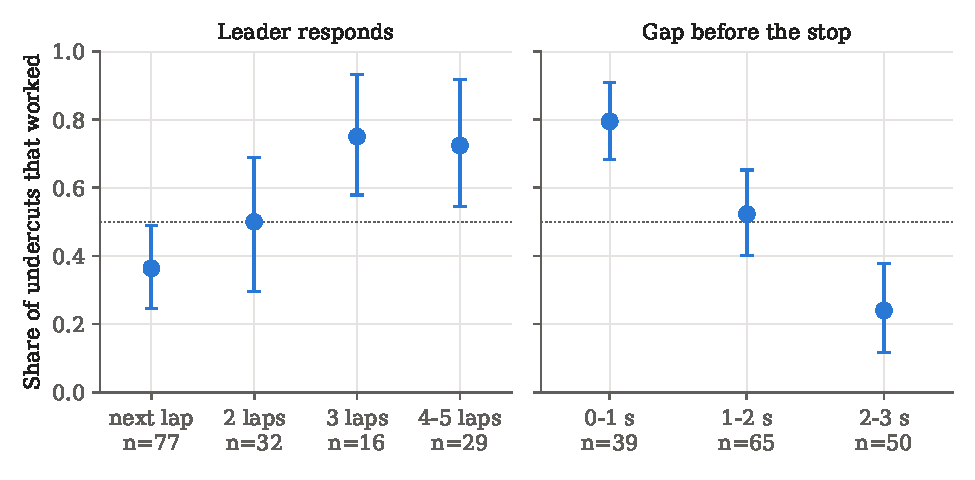
\includegraphics[width=\linewidth]{fig2_rates.pdf}
\caption{Share of undercut attempts that worked in 2023--25, by how many laps later the leader pitted (left) and by the gap before the chaser's stop (right). Bars are 95\% race-bootstrap confidence intervals; $n$ is the number of attempts. The dotted line marks 50\%.}
\label{fig:rates}
\end{figure}

Table~\ref{tab:odds} shows the logistic regression. Holding the other factors fixed, each extra second of gap multiplied the odds of success by 0.28 (95\% CI 0.15--0.51), a 72\% drop. Compared with a next-lap response, a response four or five laps later multiplied the odds by 5.4 (CI 1.8--16.5). Tyre age also mattered: each lap that the leader's tyres were older than the chaser's raised the odds by 15\% (CI 3--28\%). So did tyre wear: at circuits where lap times rose 0.01~s more per lap of tyre age, the odds were 18\% higher (CI 5--32\%). The pit-lane time loss and the choice of compound made no clear difference.

\begin{table}[t]
\centering
\caption{Logistic regression of undercut success, 2023--25 (154 attempts, 41 races). Odds ratios with 95\% confidence intervals from race-clustered standard errors. Reference levels: next-lap response; chaser moved to a harder compound.}
\label{tab:odds}
% source: results/rq1_odds.csv
\begin{tabular}{lccc}
\toprule
Factor & Odds ratio & 95\% CI & $p$ \\
\midrule
Gap before the stop (per s) & 0.28 & 0.15--0.51 & $<0.001$ \\
Leader responds 2 laps later & 1.57 & 0.62--3.98 & 0.34 \\
Leader responds 3 laps later & 6.97 & 0.89--54.8 & 0.07 \\
Leader responds 4--5 laps later & 5.45 & 1.80--16.5 & 0.003 \\
Tyre-age difference (per lap) & 1.15 & 1.03--1.28 & 0.01 \\
Same compound (vs harder) & 0.70 & 0.24--2.08 & 0.52 \\
Softer compound (vs harder) & 0.95 & 0.32--2.84 & 0.93 \\
Pit loss (per s) & 1.06 & 0.94--1.20 & 0.37 \\
Tyre wear (per 0.01 s/lap) & 1.18 & 1.05--1.32 & 0.005 \\
\bottomrule
\end{tabular}
\end{table}

Figure~\ref{fig:lookup} turns the model into a lookup chart for an average race, read as ``if the leader responds after this many laps''. With a next-lap response, the undercut is better than even only from about 1.2~s or closer: the model gives 71\% at 0.5~s, 57\% at 1.0~s, 41\% at 1.5~s and 27\% at 2.0~s. If the leader waits three laps or more, the chance at 2.0~s rises to 67--72\%. % source: results/rq1_lookup.csv (compound held at "harder")
The ``striking range'' of about two seconds that commentators describe \citep{palmer2019singapore} is therefore a range in which an undercut is possible, but likely only if the leader is slow to respond.

\begin{figure}[t]
\centering
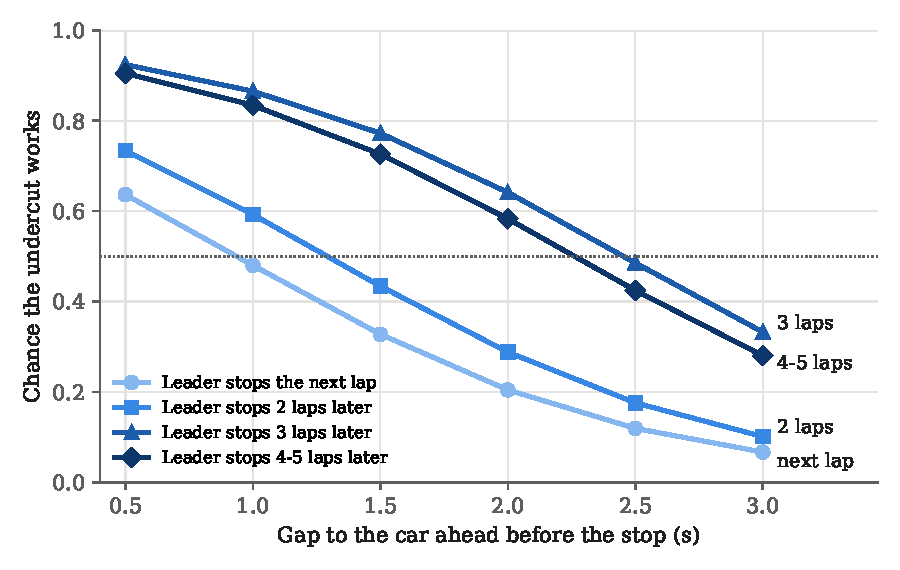
\includegraphics[width=0.9\linewidth]{fig1_lookup.pdf}
\caption{Predicted chance that an undercut works, by the gap before the chaser's stop and how many laps later the leader pits. From the logistic regression in Table~\ref{tab:odds}, with tyre-age difference, pit loss and tyre wear at their 2023--25 medians and the chaser moving to a harder compound, the most common choice.}
\label{fig:lookup}
\end{figure}

The results hold up under the robustness checks. % source: results/rq1_sensitivity.csv
The odds ratio for each second of gap was 0.31 (CI 0.12--0.79) with a 2~s window, 0.38 (0.29--0.51) with a 5~s window, 0.23 (0.12--0.44) when the outcome was checked a lap later, and 0.26 (0.14--0.48) with the relaxed green-flag rule. The odds ratio for a four-to-five-lap response ranged from 5.4 to 10.4. Success rates moved as expected with the window: 63\% within 2~s, 37\% within 5~s.

\subsection{Where the undercut's time comes from}
% source: results/mechanism.csv, analysis output (stop_diff > 3 s: 17 attempts, 88% worked)
Figure~\ref{fig:mech} splits each attempt's swing into the stops and the tyre phase, for the 153 attempts in which both stops' time loss could be measured. % source: results/mechanism.csv, analysis output (stop_diff > 3 s: 17 attempts, 15 worked)
Successful undercuts gained 6.0~s on average: 4.2~s in the tyre phase and 1.8~s because the leader's stop cost more than the chaser's (medians 4.0~s and 1.1~s). Failed undercuts lost 1.5~s: the tyre phase gained only 0.3~s, and the chaser's own stop cost 1.8~s more than the leader's (medians 0.1~s and $-1.1$~s). Of the 7.5~s average difference between successes and failures, 3.6~s (about half) came from the stops and 3.9~s from the tyre phase. A few very slow stops pull the stop averages away from the medians: in the 17 attempts where the leader's stop was more than 3~s slower than the chaser's, 15 undercuts worked (88\%). Rejoining close behind another car was about equally common in successes and failures (26\% and 22\%).

\begin{figure}[t]
\centering
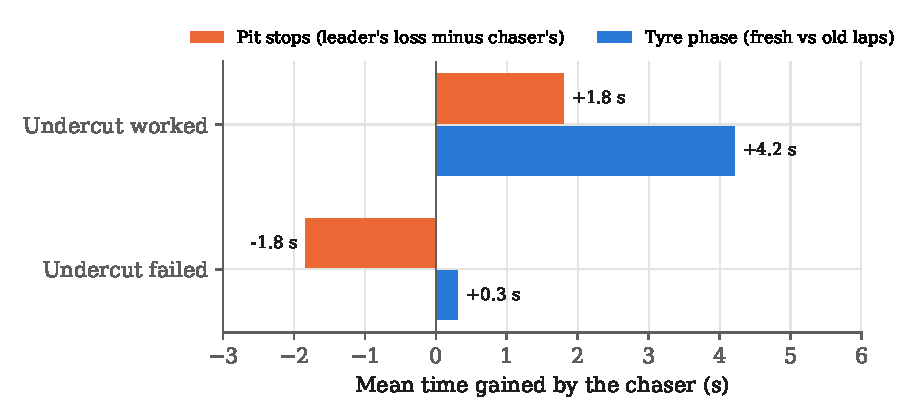
\includegraphics[width=0.9\linewidth]{fig4_mechanism.pdf}
\caption{Mean time the chaser gained on the leader, split into the pit stops (the leader's stop time loss minus the chaser's) and the tyre phase (everything else between the lap before the chaser's stop and the check lap). 2023--25, the 76 successful and 77 failed attempts in which both stops' time loss could be measured.}
\label{fig:mech}
\end{figure}

\subsection{RQ2: Does a model beat the rule of thumb?}
% source: results/rq2_rule.csv, rq2_loso.csv, rq2_2026.csv, rq2_diffs.csv
Read as a yes/no prediction, the rule of thumb is right 67\% of the time in 2023--25. When it said the undercut would work, it did 64\% of the time ($n=92$); when it said it would fail, 29\% still worked ($n=62$). The calibrated rule shows that the margin carries real information (each extra second of margin multiplies the odds by 1.51, CI 1.23--1.86) but that its 50/50 point is uncertain. With the fresh-tyre laps counted as in the rule above, an attempt is a coin flip at a margin of 1.0~s (95\% CI $-0.1$ to 1.9~s); leaving the cold out-lap out of the count moves this to $-0.3$~s (CI $-1.3$ to 0.6~s). % source: results/rq2_rule.csv
Where exactly the rule's threshold should sit therefore depends on how the fresh-tyre gain is counted, and our data cannot pin it down.

\begin{figure}[t]
\centering
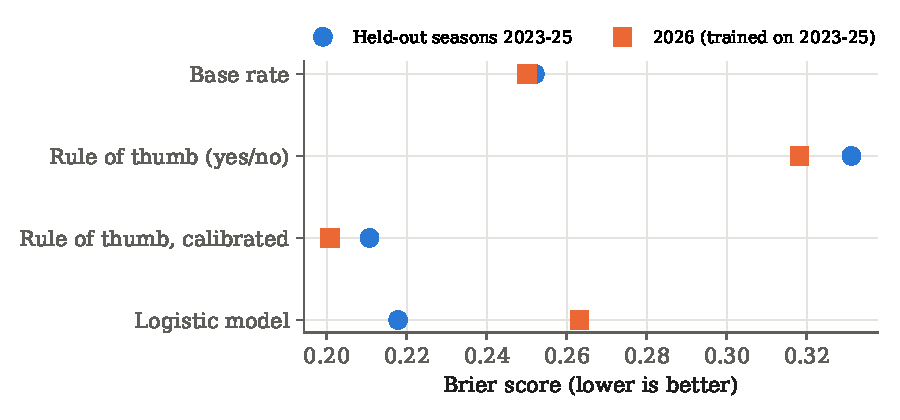
\includegraphics[width=0.9\linewidth]{fig3_models.pdf}
\caption{Brier score of four predictions of whether an undercut works (lower is better). Circles: each 2023--25 season predicted by a model fitted on the other two (154 attempts). Squares: 2026 predicted by a model fitted on 2023--25 (22 attempts).}
\label{fig:models}
\end{figure}

Figure~\ref{fig:models} and Table~\ref{tab:rq2} compare the four methods on seasons they were not fitted on. The yes/no rule is about as accurate as the fitted methods (67\%) but has the worst Brier score (0.331), worse even than predicting the base rate for everyone (0.252; difference $+0.079$, CI $+0.009$ to $+0.145$), because it is confidently wrong a third of the time. Calibrating it fixes that: the calibrated rule had a Brier score of 0.211, better than the base rate (difference $-0.041$, CI $-0.073$ to $-0.012$). The full logistic model, with ten fitted parameters instead of two, did no better (0.218; difference from the calibrated rule $+0.007$, CI $-0.030$ to $+0.046$). It was the best method when 2023 was held out but scored worse than the base rate when 2025 was held out (0.287 vs 0.253). % source: results/rq2_loso.csv On 2026 the pattern was the same: the calibrated rule scored 0.201 and the full model 0.263.

\begin{table}[t]
\centering
\caption{Out-of-sample performance. Leave one season out over 2023--25 (pooled, 154 attempts) and a 2023--25 model applied to 2026 (22 attempts).}
\label{tab:rq2}
% source: results/rq2_loso.csv (pooled), results/rq2_2026.csv
\begin{tabular}{lcccc}
\toprule
 & \multicolumn{2}{c}{2023--25, season held out} & \multicolumn{2}{c}{2026} \\
Method & Brier & Accuracy & Brier & Accuracy \\
\midrule
Base rate & 0.252 & 0.47 & 0.250 & 0.36 \\
Rule of thumb (yes/no) & 0.331 & 0.67 & 0.318 & 0.68 \\
Rule of thumb, calibrated & 0.211 & 0.68 & 0.201 & 0.73 \\
Logistic model & 0.218 & 0.67 & 0.263 & 0.64 \\
\bottomrule
\end{tabular}
\end{table}

\subsection{RQ3 (exploratory): Did 2026 change the undercut?}
% source: results/rq3_rate.csv, rq3_odds.csv, rq3_calibration.csv, rq3_by_delay.csv
In 2026, 8 of 22 attempts (in 10 races) worked: 36\%, against 50\% in 2023--25. The difference, $-14$ percentage points, has a 95\% CI of $-36$ to $+3$ points. With the other factors held fixed, a 2026 indicator gave an odds ratio of 0.34 (CI 0.11--1.00, $p=0.049$), and the 2023--25 model predicted an average success rate of 56\% for the 2026 attempts, against the 36\% that happened. Leaders also responded faster: 14 of the 22 responses (64\%) came on the next lap, against 77 of 154 (50\%) before, and of those next-lap cases only 3 of 14 worked (21\%). With so few attempts, these are hints rather than findings.

\begin{figure}[t]
\centering
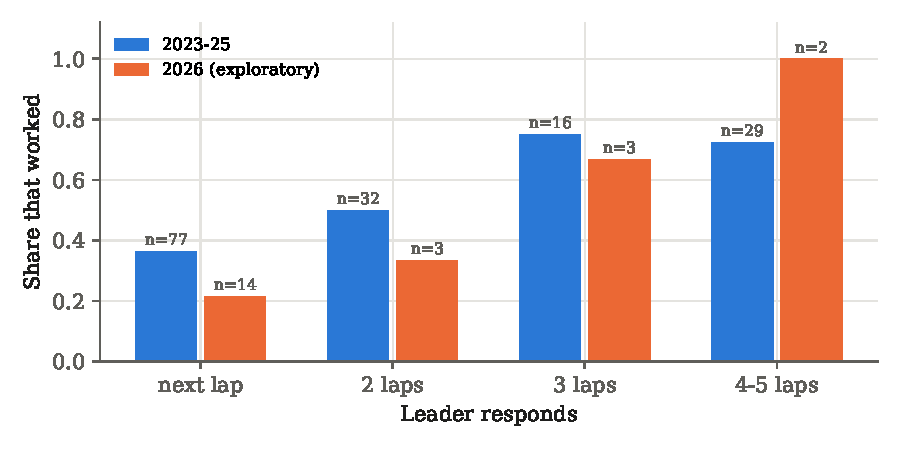
\includegraphics[width=0.9\linewidth]{fig5_2026.pdf}
\caption{Share of undercut attempts that worked, by response delay, in 2023--25 and in 2026 (exploratory; $n$ above each bar).}
\label{fig:2026}
\end{figure}

\subsection{RQ4 (exploratory): What kind of team or car closes the gap?}
% source: results/rq4_splits.csv, rq4_odds.csv, rq4_prepace.csv, rq4_prepace_split.csv, rq4_checks.csv, rq4_team_test.csv, rq4_teams.csv
Faster cars did better at first sight: when the chaser's team was the faster one over the season's other races, 58\% of its undercuts worked ($n=69$), against 44\% when it was not ($n=85$). But faster cars also tended to start closer (correlation $-0.17$ between the pace advantage and the gap), and once the gap and the response delay were in the model, pace added nothing: an odds ratio of 1.00 per 0.1~s a lap (CI 0.89--1.13). Pace on the day, from the laps before the attempt, told the same story (59\% vs 42\% raw; odds ratio 1.01 per 0.1~s a lap, CI 0.86--1.19, $n=146$). Neither a car's tyre wear (odds ratio 1.00 per 0.01~s a lap, CI 0.66--1.50) nor its team's pit-crew record (1.65 per second, CI 0.70--3.86) was clearly linked to success. The crew record did not even predict how the attempt's own stops went (correlation 0.07 with the stop difference), so the slow stops that decide some undercuts look like one-off events rather than a team trait.

Which team was being undercut did matter. Adding the leader's team to a gap-and-delay model improved it ($p=0.017$); adding the chaser's team did so only weakly ($p=0.06$). Figure~\ref{fig:teams} shows the raw rates. Undercuts against Aston Martin worked 4 times in 19, against Mercedes 5 in 16 and against Ferrari 6 in 17, but against Alpine 11 in 13, Racing Bulls 12 in 16 and Sauber/Audi 13 in 18. As the chaser, Haas succeeded 13 times in 16 and Sauber/Audi 2 times in 13. Every team has fewer than 25 attempts, so the intervals are wide.

\begin{figure}[t]
\centering
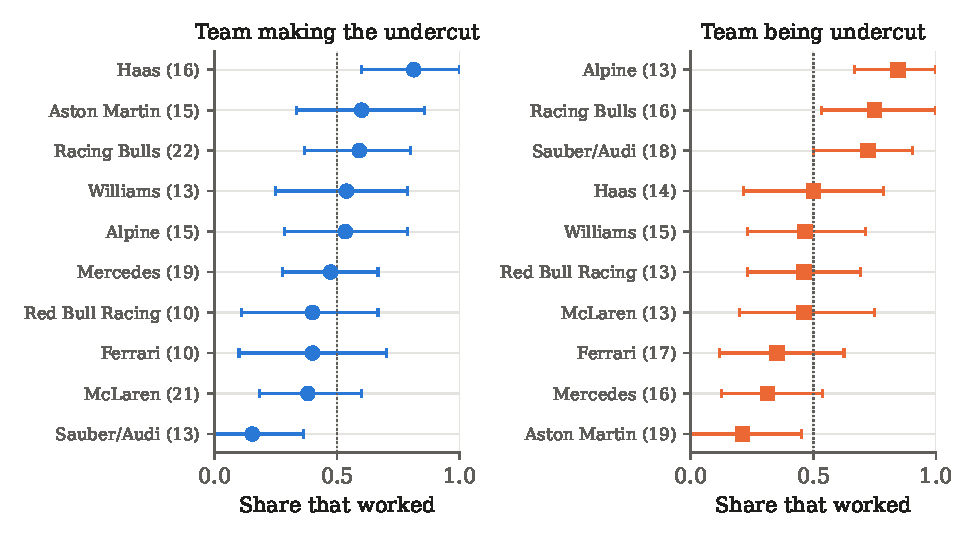
\includegraphics[width=0.95\linewidth]{fig6_teams.pdf}
\caption{Share of undercut attempts that worked, by the team making the undercut (left) and the team being undercut (right), 2023--25 (exploratory). Number of attempts in brackets; bars are 95\% race-bootstrap intervals. Each team's cars changed over the three seasons.}
\label{fig:teams}
\end{figure}

\section{Discussion}

\todo{AUTHOR: write this section in your own words (about 600--900 words). Prompts:
(1) What is the single most useful thing a fan or a strategist should take from Figure~\ref{fig:lookup}? Why is the yes/no rule overconfident, and why is its 50/50 point so sensitive to whether the out-lap counts? Think about cold tyres on the out-lap, the pit-lane exit, or the leader pushing on its in-lap.
(2) The leader's response delay matters as much as the gap. What does that suggest about who controls an undercut, the chaser or the leader? When would a leader choose not to respond on the next lap? (Remember that the leader chooses its delay after seeing the chaser stop, so this is an association, not proof of cause.)
(3) A simple two-number rule predicted as well as the full model. Why might that be, given 154 attempts? What does it mean for teams or broadcasters?
(4) About half of the difference between successful and failed undercuts came from pit-stop execution. How does that change how you would judge a strategy call after the race?
(5) 2026: success fell and leaders responded faster. What about the new cars or tyres could explain it, and why should readers be careful with 22 attempts?
(6) How do these results relate to the race simulations and game-theory models cited in the Introduction?
(7) RQ4: a faster car wins more undercuts only because it starts closer, and pit-crew records do not predict the stops. Yet the team being undercut seems to matter. What could some teams be doing differently when they defend (think about tyre warm-up, out-lap pace, or how they manage the gap before the stop)? Why should you be careful with about 15 attempts per team and six exploratory tests?}

\subsection{Limitations}
The sample is modest: 154 attempts in 2023--25 and 22 in 2026, so several estimates, especially for three-lap responses and for 2026, have wide intervals. We use only dry races and attempts in which every lap of the stop window was fully green; undercuts under safety cars, which follow different logic, are excluded, and so are attempts with a local yellow flag on any lap of the window. The response delay is chosen by the leader after the chaser stops, so its odds ratios describe association, not the effect of an assigned delay. The definition requires the leader to respond within five laps. Cases where the leader stayed out longer are a different strategic situation (often a different number of stops) and are not modelled. The race features are medians over other cars, so they describe the race, not the exact tyres of the two cars involved, and tyre wear is measured net of fuel burn. The fresh-tyre gain behind the rule of thumb is one reasonable estimator among several, and the rule's break-even point moves by more than a second depending on whether the out-lap is counted; a team with tyre-model data would estimate it better. The analysis uses only races already in the local data cache (to round 17 of 2026), because the FastF1 timing archive began requiring authentication in October 2026. In RQ4, team results pool three seasons in which each team's car changed, and a crew's stop loss measured from lap times includes the driver's in-lap and out-lap, not only the time stationary. Finally, the analysis describes what happened when teams chose to undercut; it cannot say what would have happened had they not.

\subsection{Reproducibility}
All code, the pre-registration tag, the decision log and every result file are at \url{https://github.com/0909yejun0909-commits/undercut}. From a FastF1 cache of the 2023--2026 races, the pipeline is: \texttt{build\_laps}, \texttt{build\_attempts}, \texttt{build\_teams}, \texttt{rq1}, \texttt{rq2}, \texttt{rq3}, \texttt{rq4} and \texttt{figures}, each run as \texttt{uv run python -m analysis.<step>}. The 52 unit tests run with \texttt{uv run pytest}.

\section{Conclusion}
\todo{AUTHOR: approve or rewrite.} Half of Formula 1's green-flag undercut attempts in 2023--25 worked. Whether one works depends mostly on two numbers, the gap before the stop and how many laps the car ahead waits before responding, and the commentators' arithmetic for combining them points the right way but, read as a yes/no call, is overconfident. Turned into a probability, the same rule predicts the outcome as well as a full statistical model. Under the 2026 rules, early evidence suggests the undercut has become harder.

\section*{Acknowledgments}
\todo{AUTHOR: approve.} The author thanks the developers of FastF1 for free access to Formula 1 timing data. AI assistance (Anthropic's Claude) was used to write analysis code and to draft parts of the text; the research question, the interpretations in the Discussion and all final decisions are the author's.

\bibliography{refs}

\end{document}
